\documentclass[a4paper,oneside,11pt]{book}

% Package dasar
\usepackage[utf8]{inputenc}     % untuk karakter UTF-8
\usepackage[T1]{fontenc}        % encoding font
\usepackage{graphicx}
\usepackage{titling}
\usepackage{titlesec}
\usepackage[backend=biber,style=ieee]{biblatex}

% Package tambahan untuk layout dan formatting
\usepackage{geometry}           % untuk margin
\usepackage{setspace}           % untuk spasi baris
\usepackage{fancyhdr}           % untuk header/footer
\usepackage{hyperref}           % untuk link dan bookmark
\usepackage{listings}           % untuk code Python
\usepackage{xcolor}             % untuk warna
\usepackage{float}              % untuk posisi gambar
\usepackage{tocloft}            % Untuk membuat daftar isi menampilkan "Bab 1. Pendahuluan" instead of "1. Pendahuluan",
\usepackage{lipsum}             % untuk lorem ipsum
\usepackage{indentfirst}        % untuk indent paragraf pertama
\usepackage{enumitem}           % untuk kustomisasi penomoran list (A., B., dst)

% Pengaturan layout
\geometry{left=3cm, right=2cm, top=2cm, bottom=2cm}
\onehalfspacing  % spasi 1.5

% Penomoran section dengan huruf kapital (A, B, C, ...)
\renewcommand{\thesection}{\Alph{section}}
\renewcommand{\thesubsection}{\thesection.\arabic{subsection}}
\renewcommand{\thesubsubsection}{\thesubsection.\arabic{subsubsection}}

% Penomoran figure mengikuti section (misal, Gambar A.1, A.2, ...)
\renewcommand{\thefigure}{\thesection.\arabic{figure}}
\makeatletter
\@addtoreset{figure}{section}
\makeatother

% Format chapter
\titleformat{\chapter}[hang]
  {\normalfont\huge\bfseries\centering}{\chaptertitlename\ \thechapter.}{1em}{}

% Format code Python
% --- VS Code-like code style (dark) ---
\definecolor{vscodeBg}{HTML}{1E1E1E}
\definecolor{vscodeFg}{HTML}{D4D4D4}
\definecolor{vscodeKeyword}{HTML}{569CD6}
\definecolor{vscodeString}{HTML}{CE9178}
\definecolor{vscodeComment}{HTML}{6A9955}
\definecolor{vscodeNumber}{HTML}{858585}
\definecolor{vscodeRule}{HTML}{3C3C3C}

\lstdefinestyle{vscode-dark}{
  language=PHP,
  basicstyle=\ttfamily\small\color{vscodeFg},
  backgroundcolor=\color{vscodeBg},
  keywordstyle=\color{vscodeKeyword}\bfseries,
  commentstyle=\color{vscodeComment},
  stringstyle=\color{vscodeString},
  numbers=left,
  numberstyle=\tiny\color{vscodeNumber},
  frame=single,
  rulecolor=\color{vscodeRule},
  breaklines=true,
  showstringspaces=false,
  columns=fullflexible,
  keepspaces=true,
  tabsize=2,
  xleftmargin=2cm,
  xrightmargin=1cm,
  captionpos=b,
  morekeywords={Route,Controller,Request,Response,Blade,Model,Migration,Artisan,middleware,Auth,extends,section,yield,csrf,foreach,endif}
}

\lstset{style=vscode-dark}

% Pengaturan hyperref
\hypersetup{
    colorlinks=true,
    linkcolor=black,
    filecolor=magenta,
    urlcolor=blue,
    citecolor=red
}

% Info dokumen
\newcommand{\Pertemuan}{1}
\newcommand{\Materi}{Unit Testing}
\title{Laporan Praktikum \\ Pengujian Perangkat Lunak\\
Pertemuan \Pertemuan\\
\Materi}
\newcommand{\NamaMahasiswa}{Muhammad Fauzan Putra Trisuladana}
\newcommand{\NIMMahasiswa}{24/538699/SV/24524}
\newcommand{\KelasMahasiswa}{A1}
\newcommand{\DosenPengampu}{Divi Galih Prasetyo Putri, S.Kom., M.Kom., Ph.D.}

\author{\NamaMahasiswa\\\NIMMahasiswa}

\begin{document}

% Jika ingin daftar pustaka muncul meskipun belum ada entri di ref.bib,
% tambahkan entri BibTeX ke file ref.bib terlebih dulu.

% Title Page
\begin{titlingpage} 
\begin{center}

\vspace{4cm} 
\begin{Large} 
\textbf{\thetitle} \\
\end{Large}
\vspace{2cm}


\includegraphics[height=8cm]{resource/lambang ugm.png}\\ 
\vspace{2cm}

\textbf{Disusun oleh:}\\[0.8em]
\begin{minipage}{0.8\textwidth}
\raggedright
\begin{large}
\begin{tabular}{@{}l@{\hspace{1.5em}}c@{\hspace{1.5em}}p{\textwidth}@{}}
Nama & : & \NamaMahasiswa \\
NIM & : & \NIMMahasiswa \\
Kelas & : & \KelasMahasiswa \\
Dosen Pengampu & : & \DosenPengampu \\
\end{tabular}
\end{large}
\end{minipage}

\vspace{2cm}
\begin{Large}
\textbf{Program Studi D-IV Teknologi Rekayasa Perangkat Lunak} \\
\textbf{Departemen Teknik Elektro dan Informatika} \\
\textbf{Sekolah Vokasi}\\
\textbf{Universitas Gadjah Mada}\\
\textbf{Yogyakarta}\\
\textbf{2026}\\
\end{Large}

\end{center}
\end{titlingpage}

% Header/Footer
\pagestyle{fancy}
\fancyhf{}            % kosongkan header/footer default
\renewcommand{\headrulewidth}{0pt} % hilangkan garis header (atas)
\renewcommand{\footrulewidth}{0pt} % pastikan tidak ada garis footer
\fancyfoot[C]{\thepage} % taruh nomor halaman di footer tengah

% Pastikan halaman dengan style 'plain' (mis. ToC/List) juga tanpa garis atas
\fancypagestyle{plain}{
  \fancyhf{}
  \renewcommand{\headrulewidth}{0pt}
  \renewcommand{\footrulewidth}{0pt}
  \fancyfoot[C]{\thepage}
}


% --- Styling Judul Daftar Isi, Gambar, dan Kode ---
\renewcommand{\cfttoctitlefont}{\hfill\normalfont\LARGE\bfseries}
\renewcommand{\cftaftertoctitle}{\hfill}
\renewcommand{\cftbeforetoctitleskip}{1em}
\renewcommand{\cftaftertoctitleskip}{1.5em}

% --- Format Bab di Daftar Isi ---
\renewcommand{\cftchappresnum}{Bab~}
\renewcommand{\cftchapaftersnum}{.}
\renewcommand{\cftchapnumwidth}{3.5em}
\renewcommand{\cftchapfont}{\bfseries}
\renewcommand{\cftchappagefont}{\bfseries}

% --- Spasi dan Estetika ---
\setlength{\cftbeforechapskip}{0.8em} % jarak antar bab
\setlength{\cftbeforesecskip}{0.2em}  % jarak antar subbab
\renewcommand{\cftsecfont}{\normalfont}
\renewcommand{\cftsubsecfont}{\normalfont}

% --- Judul Lokal ---
\renewcommand{\contentsname}{\centering Daftar Isi}
\renewcommand{\listfigurename}{\centering Daftar Gambar}
\renewcommand{\lstlistlistingname}{\centering Daftar Kode}

% --- Gaya Daftar Gambar dan Daftar Kode ---
\renewcommand{\cftloftitlefont}{\hfill\normalfont\LARGE\bfseries}
\renewcommand{\cftafterloftitle}{\hfill}

\tableofcontents

\newpage
% Daftar Gambar
\listoffigures

\newpage
% Daftar Listing
\lstlistoflistings

% --- Halaman Laporan Pertemuan (seperti contoh gambar) ---
% Tidak pakai \chapter agar bisa menyatu dengan halaman sebelumnya.
\newpage
\begin{center}
\textbf{\LARGE Pertemuan \Pertemuan\\
{[{\Materi}]}}
\end{center}

\section{Tujuan Praktikum}
\begin{enumerate}
    \item Mahasiswa mampu memahami unit testing
    \item Mahasiswa mampu menggunakan JUnit untuk melakukan unit testing pada aplikasi Java
    \item Mahasiswa mampu menulis dan menjalankan test case menggunakan JUnit
\end{enumerate}

%contoh gambar dan kode
% \begin{figure}[H]
%     \centering
%     \includegraphics[width=0.5\textwidth]{resource/contoh-gambar.png}
%     \caption{Contoh Gambar}
%     \label{fig:contoh-gambar}
% \end{figure}

% \begin{lstlisting}[language=php, caption={Contoh Kode Python}, label={lst:contoh-kode}]
% def hello_world():
%     print("Hello, World!")
% \end{lstlisting}

\section{Hasil dan Pembahasan}
\subsection{Persiapan Praktikum}
\par Pada tahap ini, saya melakukan instalasi dan konfigurasi lingkungan pengembangan untuk praktikum unit testing menggunakan JUnit. Saya memastikan bahwa Java Development Kit (JDK) sudah terpasang dengan benar, serta karena saya ingin menggunakan vscode sebagai code editor, saya juga menginstal ekstensi Java Extension Pack yang menyediakan dukungan untuk pengembangan Java, termasuk fitur untuk menjalankan dan menulis test case dengan JUnit. Setelah itu, Saya mengintall maven untuk bisa menggunakan JUnit

\par Setelah Semua proses instalasi selesai saya membuat project Java baru menggunakan Maven, seperti pada gambar \ref{fig:project-setup}. Saya memilih yang tanpa archetype untuk membuat struktur proyek yang sederhana dan siap digunakan untuk pengembangan aplikasi Java.

\begin{figure}[H]
    \centering
    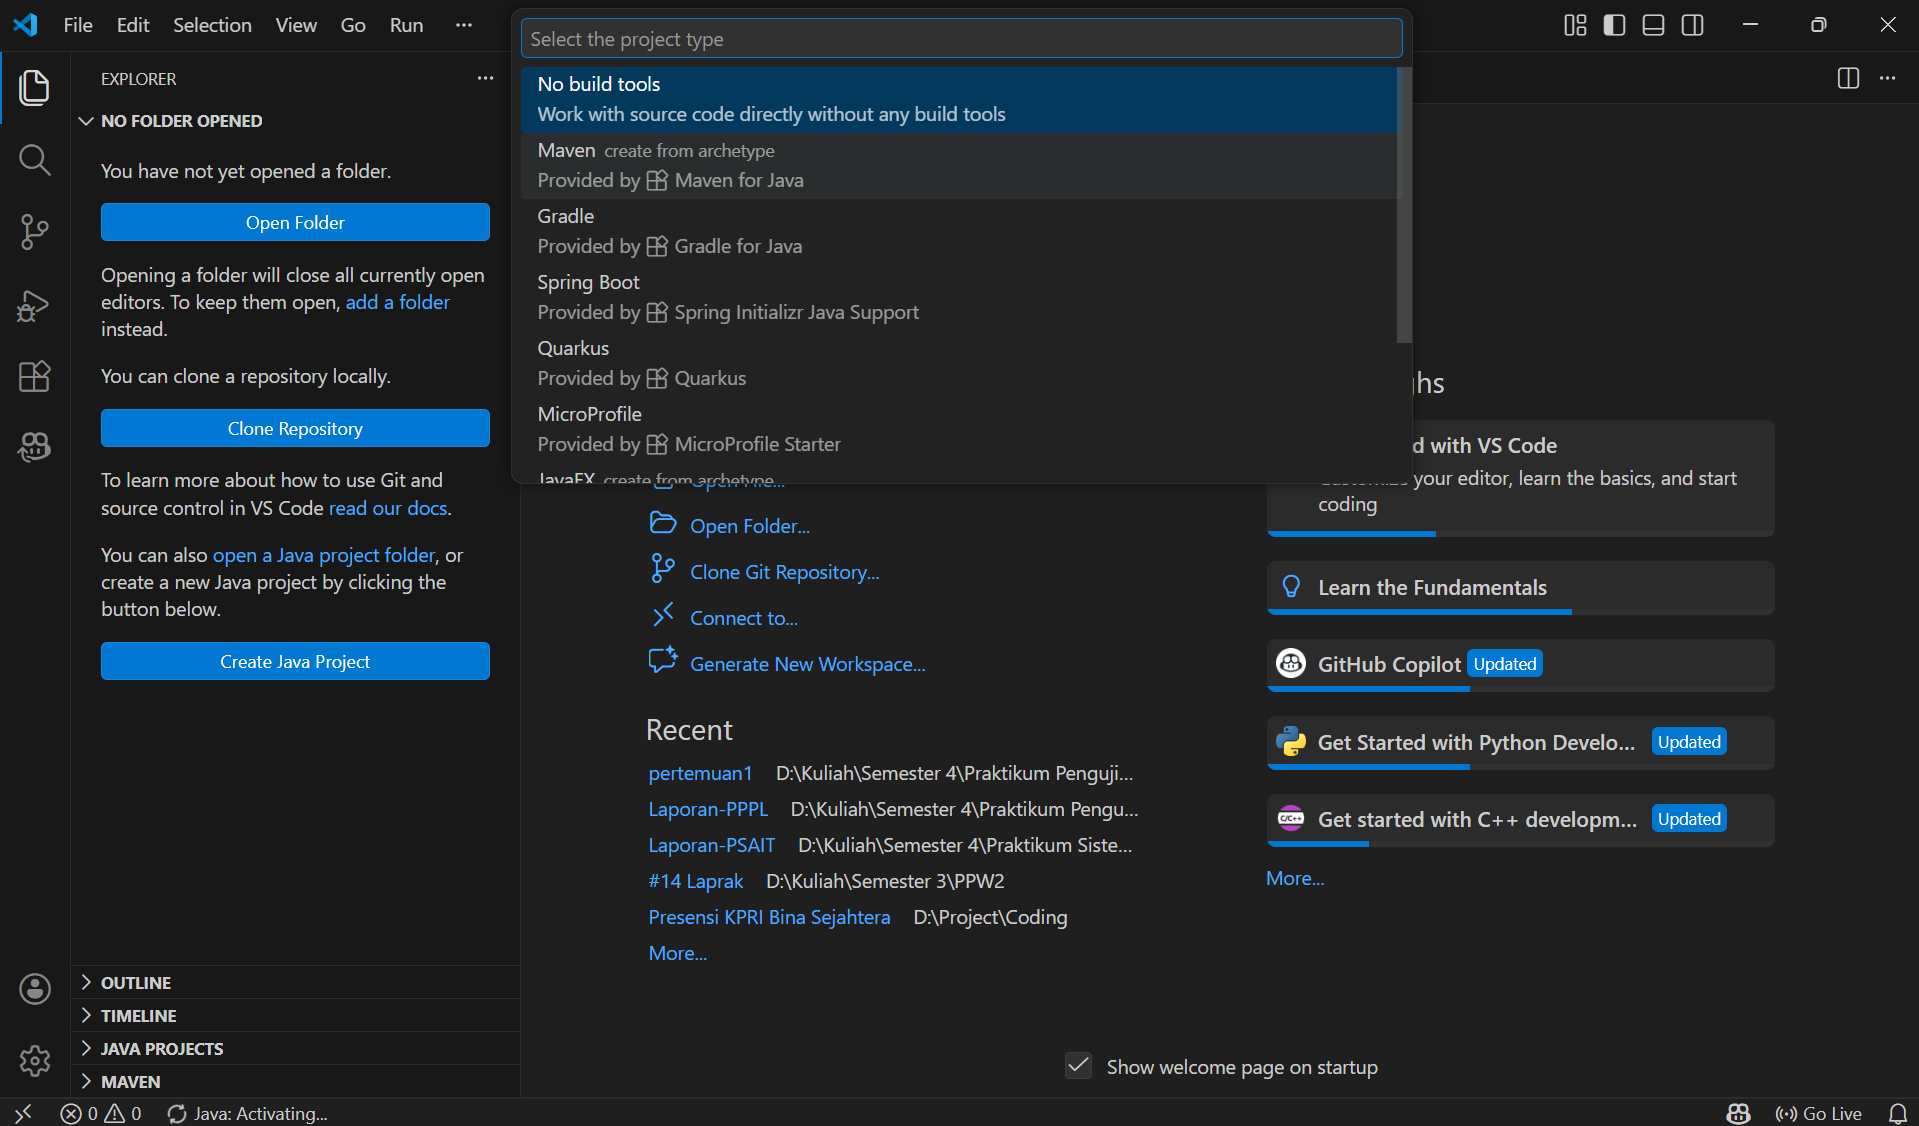
\includegraphics[width=0.8\textwidth]{resource/instalasi-maven.png}
    \caption{Setup Project Java dengan Maven}
    \label{fig:project-setup}
\end{figure}

\par Setelah project berhasil dibuat, saya menambahkan dependensi JUnit ke dalam file pom.xml untuk bisa menggunakan JUnit dalam proyek Java saya. Saya menambahkan kode berikut ke dalam bagian <dependencies> di pom.xml:
\begin{lstlisting}[language=xml, caption={Menambahkan Dependensi JUnit di pom.xml}, label={lst:dependensi-junit}]
<dependencies>
    <!-- Source: https://mvnrepository.com/artifact/org.junit.jupiter/junit-jupiter -->
    <dependency>
        <groupId>org.junit.jupiter</groupId>
        <artifactId>junit-jupiter</artifactId>
        <version>5.10.5</version>
        <scope>test</scope>
    </dependency>
</dependencies>
\end{lstlisting}
\par Kode di atas \ref{lst:dependensi-junit} saya dapatkan dari situs mvnrepository.com, yang merupakan sumber terpercaya untuk mencari dependensi Java. Saya mengetikkan kata kunci "JUnit" di situs tersebut, lalu memilih JUnit Jupiter (Agregator) \ref{fig:dependensi-junit}.

\begin{figure}[H]
    \centering
    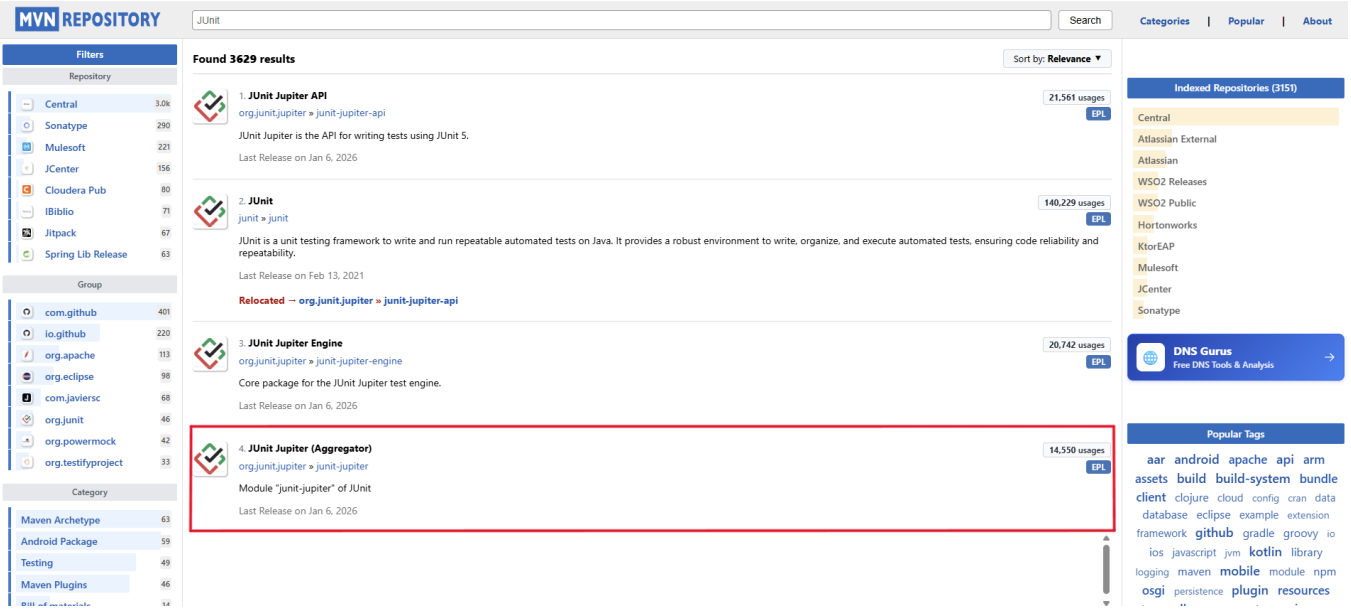
\includegraphics[width=0.8\textwidth]{resource/dependensi-junit.png}
    \caption{Mencari dependensi JUnit di mvnrepository.com}
    \label{fig:dependensi-junit}
\end{figure}

\par Kemudian saya memilih versi 5.10.5 dari JUnit Jupiter (Agregator) karena merupakan versi yang stabil dan memiliki fitur lengkap untuk pengujian unit di Java. Saya menyalin kode dependensi yang disediakan di situs tersebut dan menempelkannya ke dalam file pom.xml proyek saya, seperti yang ditunjukkan pada listing \ref{lst:dependensi-junit}.
\begin{figure}[H]
    \centering
    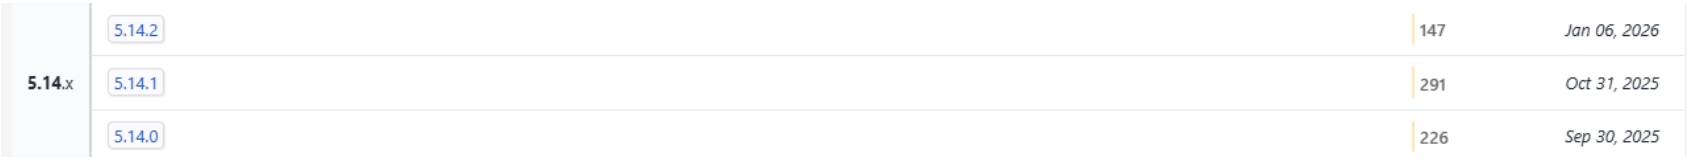
\includegraphics[width=0.8\textwidth]{resource/versi-junit.png}
    \caption{Memilih versi JUnit Jupiter (Agregator)}
    \label{fig:versi-junit}
\end{figure}

\par Setelah menambahkan dependensi, saya melakukan build proyek \ref{fig:build-project} untuk memastikan bahwa semua dependensi terunduh dengan benar dan proyek siap digunakan untuk pengembangan lebih lanjut.
\begin{figure}[H]
    \centering
    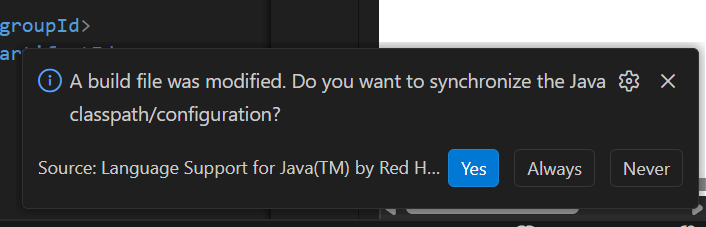
\includegraphics[width=0.8\textwidth]{resource/build-project.png}
    \caption{Melakukan Build Proyek setelah Menambahkan Dependensi}
    \label{fig:build-project}
\end{figure}

\subsection{Hasil Pengujian dengan JUnit}

\par Pada tahap ini, saya melakukan pengujian unit menggunakan JUnit 5 pada kelas \textit{Wallet} yang saya buat di proyek Maven. Saya akan menympan list cards dan cash sebagai atribut utama untuk menyimpan data kartu dan uang tunai. Saya juga menambahkan method untuk mengelola kedua atribut tersebut, seperti \textit{addCards}, \textit{withdrawCards}, \textit{addCash}, \textit{withdrawCash}, serta method untuk mengambil data dan menghitung total saldo.

\par Berikut merupakan kode implementasi kelas \textit{Wallet} yang menjadi objek pengujian pada praktikum ini.
\begin{lstlisting}[language=Java, caption={Potongan implementasi kelas Wallet (sumber: Wallet.java)}, label={lst:wallet-impl}]
package com.example;

import java.util.ArrayList;
import java.util.Collections;
import java.util.List;

public class Wallet {
    private String owner;
    private final List<String> cards;
    private final List<Double> cash;

    public Wallet() {
        this.cards = new ArrayList<>();
        this.cash = new ArrayList<>();
    }

    public Wallet(String owner) {
        this();
        setOwner(owner);
    }

    public void setOwner(String owner) {
        if (owner == null) {
            throw new IllegalArgumentException("owner tidak boleh null");
        }
        this.owner = owner;
    }

    public String getOwner() {
        return owner;
    }

    public void addCards(List<String> cards) {
        if (cards == null) {
            throw new IllegalArgumentException("cards tidak boleh null");
        }
        for (String card : cards) {
            if (card == null) {
                throw new IllegalArgumentException("card tidak boleh null");
            }
        }
        this.cards.addAll(cards);
    }

    public void withdrawCards(List<String> cards) {
        if (cards == null) {
            throw new IllegalArgumentException("cards tidak boleh null");
        }
        for (String card : cards) {
            if (card == null) {
                throw new IllegalArgumentException("card tidak boleh null");
            }
            if (this.cards.contains(card)) {
                this.cards.remove(card);
            }
        }
    }

    public List<String> getCards() {
        return Collections.unmodifiableList(new ArrayList<>(cards));
    }

    public void addCash(List<Double> cash) {
        if (cash == null) {
            throw new IllegalArgumentException("cash tidak boleh null");
        }
        for (Double amount : cash) {
            if (amount == null) {
                throw new IllegalArgumentException("amount tidak boleh null");
            }
            if (amount <= 0) {
                throw new IllegalArgumentException("amount harus > 0");
            }
        }
        this.cash.addAll(cash);
    }

    public void withdrawCash(List<Double> cash) {
        if (cash == null) {
            throw new IllegalArgumentException("cash tidak boleh null");
        }
        for (Double amount : cash) {
            if (amount == null) {
                throw new IllegalArgumentException("amount tidak boleh null");
            }
            if (this.cash.contains(amount)) {
                this.cash.remove(amount);
            }
        }
    }

    public List<Double> getCash() {
        return Collections.unmodifiableList(new ArrayList<>(cash));
    }

    public double getCashAmount() {
        double total = 0;
        for (Double amount : cash) {
            total += amount;
        }
        return total;
    }
}
\end{lstlisting}

\par Berikut metod-method yang ada pada kelas \textit{Wallet} berdasarkan Listing \ref{lst:wallet-impl} (baris dihitung dari baris 1 pada listing itu):
\begin{enumerate}
    \item \textbf{Constructor \textit{Wallet()} (Listing \ref{lst:wallet-impl} baris 12--15)} dibuat untuk menginisialisasi atribut list \textit{cards} dan \textit{cash} sebagai \textit{ArrayList} kosong. Dengan demikian, objek \textit{Wallet} selalu memiliki list yang siap dipakai dan tidak bernilai null.
    \item \textbf{Constructor \textit{Wallet(String owner)} (Listing \ref{lst:wallet-impl} baris 17--20)} dibuat untuk menginisialisasi objek sekaligus menetapkan nilai \textit{owner}. Constructor ini memanggil constructor default (\textit{this()}) untuk menginisialisasi list, lalu memanggil \textit{setOwner(owner)} agar validasi owner tetap digunakan.
    \item \textbf{Method \textit{setOwner(String owner)} (Listing \ref{lst:wallet-impl} baris 22--27)} digunakan untuk mengubah nilai \textit{owner}. Method ini melakukan validasi: jika parameter \textit{owner} bernilai null maka akan melempar \textit{IllegalArgumentException} dengan pesan \textit{"owner tidak boleh null"}.
    \item \textbf{Method \textit{getOwner()} (Listing \ref{lst:wallet-impl} baris 29--31)} digunakan untuk mendapatkan nilai \textit{owner} yang tersimpan pada objek.
    \item \textbf{Method \textit{addCards(List<String> cards)} (Listing \ref{lst:wallet-impl} baris 33--43)} digunakan untuk menambahkan beberapa kartu sekaligus ke dalam list \textit{cards}. Method ini menolak input null (melempar \textit{IllegalArgumentException} \textit{"cards tidak boleh null"}) dan menolak elemen kartu yang null (melempar \textit{IllegalArgumentException} \textit{"card tidak boleh null"}). Jika valid, seluruh elemen akan ditambahkan dengan \textit{addAll}.
    \item \textbf{Method \textit{withdrawCards(List<String> cards)} (Listing \ref{lst:wallet-impl} baris 45--57)} digunakan untuk menghapus beberapa kartu sekaligus dari list \textit{cards}. Method ini menolak input null dan elemen null sama seperti \textit{addCards}. Untuk setiap kartu, method hanya menghapus jika kartu tersebut ada di dalam list (dicek dengan \textit{contains}), sehingga kartu yang tidak ditemukan akan diabaikan tanpa error.
    \item \textbf{Method \textit{getCards()} (Listing \ref{lst:wallet-impl} baris 59--61)} digunakan untuk mengambil daftar kartu yang ada. Method ini mengembalikan \textit{snapshot} dalam bentuk list read-only dengan \textit{Collections.unmodifiableList(new ArrayList<>(cards))}, sehingga list yang diterima dari luar tidak bisa dimodifikasi dan tidak langsung memengaruhi data internal.
    \item \textbf{Method \textit{addCash(List<Double> cash)} (Listing \ref{lst:wallet-impl} baris 63--76)} digunakan untuk menambahkan beberapa nominal uang sekaligus ke dalam list \textit{cash}. Method ini menolak input null (\textit{"cash tidak boleh null"}), menolak elemen nominal null (\textit{"amount tidak boleh null"}), dan menolak nominal \textit{<= 0} (\textit{"amount harus > 0"}). Jika valid, seluruh nominal ditambahkan dengan \textit{addAll}.
    \item \textbf{Method \textit{withdrawCash(List<Double> cash)} (Listing \ref{lst:wallet-impl} baris 78--90)} digunakan untuk menghapus beberapa nominal uang dari list \textit{cash}. Method ini menolak input null dan elemen nominal null. Untuk setiap nominal, method hanya menghapus jika nominal tersebut ada pada list, sehingga nominal yang tidak ditemukan akan diabaikan tanpa error.
    \item \textbf{Method \textit{getCash()} (Listing \ref{lst:wallet-impl} baris 92--94)} digunakan untuk mengambil daftar nominal uang yang tersimpan. Sama seperti \textit{getCards}, method ini mengembalikan \textit{snapshot} read-only agar data internal tidak dapat dimodifikasi langsung dari luar.
    \item \textbf{Method \textit{getCashAmount()} (Listing \ref{lst:wallet-impl} baris 96--102)} digunakan untuk menghitung total saldo uang tunai. Method ini menjumlahkan seluruh elemen pada list \textit{cash} dan mengembalikan hasil penjumlahan tersebut sebagai nilai \textit{double}.
\end{enumerate}

\par Setelah implementasi dibuat, saya menyusun kelas \textit{unit test} \textit{WalletTest} menggunakan beberapa jenis assert seperti \textit{assertAll}, \textit{assertEquals}, \textit{assertTrue}, \textit{assertThrows}, dan \textit{assertDoesNotThrow}. Pengujian saya bagi menjadi dua bagian besar: pengelolaan kartu (cards) dan pengelolaan uang tunai (cash).

\subsubsection{Pengujian Inisialisasi Objek}
\par Pengujian pertama memastikan bahwa objek \textit{Wallet} dalam kondisi awal yang benar ketika menggunakan constructor tanpa parameter. Saya memeriksa bahwa list kartu dan list uang tidak bernilai null, masih kosong, serta total saldo yang dihitung oleh \textit{getCashAmount} bernilai 0.
\begin{lstlisting}[language=Java, caption={Implementasi kelas WalletTest (sumber: WalletTest.java)}, label={lst:test-initial-state}]
package com.example;

import org.junit.jupiter.api.Test;

import static org.junit.jupiter.api.Assertions.*;

import java.util.Arrays;
import java.util.List;

class WalletTest {

    @Test
    void testInitialState() {
        Wallet wallet = new Wallet();
        assertAll(
                () -> assertNotNull(wallet.getCards()),
                () -> assertNotNull(wallet.getCash()),
                () -> assertTrue(wallet.getCards().isEmpty()),
                () -> assertTrue(wallet.getCash().isEmpty()),
                () -> assertEquals(0.0, wallet.getCashAmount(), 0.0001)
        );
    }

    @Test
    void testSetAndGetOwner() {
        Wallet wallet = new Wallet();
        wallet.setOwner("Budi");
        assertEquals("Budi", wallet.getOwner());
    }

    @Test
    void testSetOwnerRejectsNull() {
        Wallet wallet = new Wallet();
        assertThrows(IllegalArgumentException.class, () -> wallet.setOwner(null));
    }

    @Test
    void testAddAndGetCards() {
        Wallet wallet = new Wallet();
        List<String> cards = Arrays.asList("Kartu1", "Kartu2");
        wallet.addCards(cards);
        assertIterableEquals(cards, wallet.getCards());
    }

    @Test
    void testGetCardsIsReadOnlySnapshot() {
        Wallet wallet = new Wallet();
        wallet.addCards(List.of("Kartu1"));

        List<String> snapshot = wallet.getCards();
        assertThrows(UnsupportedOperationException.class, () -> snapshot.add("Kartu2"));
        assertIterableEquals(List.of("Kartu1"), wallet.getCards());
    }

    @Test
    void testAddCardsRejectsNullListAndNullItems() {
        Wallet wallet = new Wallet();
        assertAll(
                () -> assertThrows(IllegalArgumentException.class, () -> wallet.addCards(null)),
                () -> assertThrows(IllegalArgumentException.class, () -> wallet.addCards(Arrays.asList("Kartu1", null)))
        );
    }

    @Test
    void testWithdrawCards() {
        Wallet wallet = new Wallet();
        wallet.addCards(Arrays.asList("Kartu1", "Kartu2", "Kartu3"));
        wallet.withdrawCards(Arrays.asList("Kartu2"));
        assertIterableEquals(Arrays.asList("Kartu1", "Kartu3"), wallet.getCards());
    }

    @Test
    void testWithdrawCardsIgnoresMissingCard() {
        Wallet wallet = new Wallet();
        wallet.addCards(Arrays.asList("Kartu1", "Kartu2"));

        assertDoesNotThrow(() -> wallet.withdrawCards(Arrays.asList("TidakAda")));
        assertIterableEquals(Arrays.asList("Kartu1", "Kartu2"), wallet.getCards());
    }

    @Test
    void testWithdrawCardsRejectsNullListAndNullItems() {
        Wallet wallet = new Wallet();
        assertAll(
                () -> assertThrows(IllegalArgumentException.class, () -> wallet.withdrawCards(null)),
                () -> assertThrows(IllegalArgumentException.class, () -> wallet.withdrawCards(Arrays.asList("Kartu1", null)))
        );
    }

    @Test
    void testAddAndGetCash() {
        Wallet wallet = new Wallet();
        List<Double> cash = Arrays.asList(1000.0, 2000.0);
        wallet.addCash(cash);
        assertIterableEquals(cash, wallet.getCash());
    }

    @Test
    void testGetCashIsReadOnlySnapshot() {
        Wallet wallet = new Wallet();
        wallet.addCash(List.of(1000.0));

        List<Double> snapshot = wallet.getCash();
        assertThrows(UnsupportedOperationException.class, () -> snapshot.add(2000.0));
        assertIterableEquals(List.of(1000.0), wallet.getCash());
    }

    @Test
    void testAddCashRejectsInvalidAmounts() {
        Wallet wallet = new Wallet();
        assertAll(
                () -> assertThrows(IllegalArgumentException.class, () -> wallet.addCash(null)),
                () -> assertThrows(IllegalArgumentException.class, () -> wallet.addCash(Arrays.asList(1000.0, null))),
                () -> assertThrows(IllegalArgumentException.class, () -> wallet.addCash(Arrays.asList(0.0))),
                () -> assertThrows(IllegalArgumentException.class, () -> wallet.addCash(Arrays.asList(-500.0)))
        );
    }

    @Test
    void testWithdrawCash() {
        Wallet wallet = new Wallet();
        wallet.addCash(Arrays.asList(1000.0, 2000.0, 5000.0));
        wallet.withdrawCash(Arrays.asList(2000.0));
        assertIterableEquals(Arrays.asList(1000.0, 5000.0), wallet.getCash());
    }

    @Test
    void testWithdrawCashIgnoresMissingAmount() {
        Wallet wallet = new Wallet();
        wallet.addCash(Arrays.asList(1000.0, 2000.0));
        wallet.withdrawCash(Arrays.asList(9999.0));
        assertIterableEquals(Arrays.asList(1000.0, 2000.0), wallet.getCash());
    }

    @Test
    void testWithdrawCashRejectsNullListAndNullItems() {
        Wallet wallet = new Wallet();
        assertAll(
                () -> assertThrows(IllegalArgumentException.class, () -> wallet.withdrawCash(null)),
                () -> assertThrows(IllegalArgumentException.class, () -> wallet.withdrawCash(Arrays.asList(1000.0, null)))
        );
    }

    @Test
    void testGetCashAmount() {
        Wallet wallet = new Wallet();
        wallet.addCash(Arrays.asList(1000.0, 2000.0, 500.0));
        assertEquals(3500.0, wallet.getCashAmount(), 0.0001);
    }
}
\end{lstlisting}

\par Berikut adalah gungsi setiap method test pada kelas \textit{WalletTest} berdasarkan Listing \ref{lst:test-initial-state} (baris dihitung dari baris 1 pada listing tersebut) dan dikelompokkan berdasarkan fungsinya:
\begin{enumerate}
    \item \textbf{Inisialisasi Objek}
    \begin{enumerate}[label=\alph*.]
        \item \textbf{testInitialState()} (Listing \ref{lst:test-initial-state} baris 12--22) menguji kondisi awal object \textit{Wallet}. Pengujian memastikan list \textit{cards} dan \textit{cash} tidak null, keduanya kosong, serta total saldo dari \textit{getCashAmount()} bernilai 0.
    \end{enumerate}

    \item \textbf{Owner}
    \begin{enumerate}[label=\alph*.]
        \item \textbf{testSetAndGetOwner()} (Listing \ref{lst:test-initial-state} baris 24--29) menguji skenario positif bahwa \textit{setOwner("Budi")} berhasil menyimpan nilai owner dan \textit{getOwner()} mengembalikan nilai yang sama.
        \item \textbf{testSetOwnerRejectsNull()} (Listing \ref{lst:test-initial-state} baris 31--35) menguji skenario negatif bahwa \textit{setOwner(null)} melempar \textit{IllegalArgumentException} sesuai validasi pada kelas \textit{Wallet}.
    \end{enumerate}

    \item \textbf{Cards (Pengelolaan Kartu)}
    \begin{enumerate}[label=\alph*.]
        \item \textbf{testAddAndGetCards()} (Listing \ref{lst:test-initial-state} baris 37--43) menguji bahwa \textit{addCards} berhasil menambahkan data kartu dan \textit{getCards()} mengembalikan isi list yang sesuai.
        \item \textbf{testGetCardsIsReadOnlySnapshot()} (Listing \ref{lst:test-initial-state} baris 45--53) menguji bahwa \textit{getCards()} mengembalikan snapshot read-only. Ketika snapshot dicoba untuk dimodifikasi, harus muncul \textit{UnsupportedOperationException}, dan isi kartu pada \textit{Wallet} tetap.
        \item \textbf{testAddCardsRejectsNullListAndNullItems()} (Listing \ref{lst:test-initial-state} baris 55--62) menguji validasi input untuk \textit{addCards}, yaitu menolak list null dan menolak elemen kartu yang bernilai null (melempar \textit{IllegalArgumentException}).
        \item \textbf{testWithdrawCards()} (Listing \ref{lst:test-initial-state} baris 64--70) menguji bahwa \textit{withdrawCards} dapat menghapus kartu yang ada pada list.
        \item \textbf{testWithdrawCardsIgnoresMissingCard()} (Listing \ref{lst:test-initial-state} baris 72--79) menguji bahwa \textit{withdrawCards} tidak menimbulkan error ketika kartu yang ditarik tidak ada (diuji dengan \textit{assertDoesNotThrow}) dan isi list kartu tetap.
        \item \textbf{testWithdrawCardsRejectsNullListAndNullItems()} (Listing \ref{lst:test-initial-state} baris 81--88) menguji validasi input untuk \textit{withdrawCards}, yaitu menolak list null dan elemen kartu null (melempar \textit{IllegalArgumentException}).
    \end{enumerate}

    \item \textbf{Cash (Pengelolaan Uang Tunai)}
    \begin{enumerate}[label=\alph*.]
        \item \textbf{testAddAndGetCash()} (Listing \ref{lst:test-initial-state} baris 90--96) menguji bahwa \textit{addCash} berhasil menambahkan nominal dan \textit{getCash()} mengembalikan isi list nominal yang sesuai.
        \item \textbf{testGetCashIsReadOnlySnapshot()} (Listing \ref{lst:test-initial-state} baris 98--106) menguji bahwa \textit{getCash()} mengembalikan snapshot read-only. Ketika snapshot dicoba untuk dimodifikasi, harus muncul \textit{UnsupportedOperationException}, dan isi cash pada \textit{Wallet} tetap.
        \item \textbf{testAddCashRejectsInvalidAmounts()} (Listing \ref{lst:test-initial-state} baris 108--117) menguji validasi input pada \textit{addCash}, yaitu menolak list null, elemen nominal null, nominal 0, dan nominal negatif (melempar \textit{IllegalArgumentException}).
        \item \textbf{testWithdrawCash()} (Listing \ref{lst:test-initial-state} baris 119--125) menguji bahwa \textit{withdrawCash} dapat menghapus nominal yang ada pada list.
        \item \textbf{testWithdrawCashIgnoresMissingAmount()} (Listing \ref{lst:test-initial-state} baris 127--133) menguji bahwa \textit{withdrawCash} mengabaikan nominal yang tidak ada tanpa error, sehingga isi list cash tetap sesuai.
        \item \textbf{testWithdrawCashRejectsNullListAndNullItems()} (Listing \ref{lst:test-initial-state} baris 135--142) menguji validasi input pada \textit{withdrawCash}, yaitu menolak list null dan elemen nominal null (melempar \textit{IllegalArgumentException}).
        \item \textbf{testGetCashAmount()} (Listing \ref{lst:test-initial-state} baris 144--149) menguji perhitungan total saldo melalui \textit{getCashAmount()} dengan menjumlahkan seluruh nominal pada list cash.
    \end{enumerate}
\end{enumerate}

\subsubsection{Pengujian Owner (Setter dan Getter)}
\par Selanjutnya, saya menguji method \textit{setOwner} dan \textit{getOwner}. Skenario positif memastikan bahwa nilai owner tersimpan dan dapat diambil kembali. Skenario negatif memastikan bahwa \textit{setOwner(null)} melempar \textit{IllegalArgumentException} sesuai validasi yang saya buat pada kelas \textit{Wallet}.

\subsubsection{Pengujian Pengelolaan Kartu (Cards)}
\par Pada bagian ini, saya menguji penambahan kartu menggunakan \textit{addCards} dan penghapusan kartu menggunakan \textit{withdrawCards}. Karena implementasi saya menerima input berbentuk \textit{List<String>}, maka saya menguji beberapa kondisi berikut:
\begin{enumerate}
    \item \textbf{Menambahkan kartu berhasil}: list kartu yang diambil melalui \textit{getCards} berisi data yang sama dengan input.
    \item \textbf{Snapshot read-only}: method \textit{getCards} mengembalikan list yang tidak bisa dimodifikasi (\textit{unmodifiableList}) sehingga penambahan elemen secara langsung akan memunculkan \textit{UnsupportedOperationException}.
    \item \textbf{Validasi input}: \textit{addCards(null)} dan list yang mengandung elemen null harus ditolak dengan \textit{IllegalArgumentException}.
    \item \textbf{Penghapusan kartu}: ketika kartu ada, kartu tersebut berhasil dihapus dari list.
    \item \textbf{Penghapusan kartu yang tidak ada}: tidak menimbulkan error (diuji menggunakan \textit{assertDoesNotThrow}) dan data tetap.
\end{enumerate}

\par Berikut salah satu contoh pengujian snapshot read-only untuk kartu.
\begin{lstlisting}[language=Java, caption={Test getCards mengembalikan snapshot read-only (sumber: WalletTest.java)}, label={lst:test-cards-readonly}]
@Test
void testGetCardsIsReadOnlySnapshot() {
    Wallet wallet = new Wallet();
    wallet.addCards(List.of("Kartu1"));

    List<String> snapshot = wallet.getCards();
    assertThrows(UnsupportedOperationException.class, () -> snapshot.add("Kartu2"));
    assertIterableEquals(List.of("Kartu1"), wallet.getCards());
}
\end{lstlisting}

\subsubsection{Pengujian Pengelolaan Uang Tunai (Cash)}
\par Pada bagian cash, saya menguji \textit{addCash}, \textit{withdrawCash}, \textit{getCash}, dan \textit{getCashAmount}. Karena uang disimpan sebagai list nominal, saya memfokuskan pengujian pada:
\begin{enumerate}
    \item \textbf{Menambahkan uang berhasil}: list cash berisi nominal yang ditambahkan.
    \item \textbf{Validasi nominal}: input null, nominal null, nominal 0, dan nominal negatif ditolak dengan \textit{IllegalArgumentException}.
    \item \textbf{Snapshot read-only}: \textit{getCash} mengembalikan list yang tidak dapat dimodifikasi.
    \item \textbf{Penarikan uang}: nominal tertentu dapat dihapus dari list ketika ada, dan jika nominal tidak ada maka diabaikan tanpa error.
    \item \textbf{Total saldo}: \textit{getCashAmount} menghitung total dengan menjumlahkan seluruh nominal yang tersimpan.
\end{enumerate}

\par Berikut contoh pengujian untuk memastikan \textit{getCashAmount} menghitung total saldo dengan benar.
\begin{lstlisting}[language=Java, caption={Test perhitungan total cash (sumber: WalletTest.java)}, label={lst:test-cash-amount}]
@Test
void testGetCashAmount() {
    Wallet wallet = new Wallet();
    wallet.addCash(Arrays.asList(1000.0, 2000.0, 500.0));
    assertEquals(3500.0, wallet.getCashAmount(), 0.0001);
}
\end{lstlisting}

\par Saya menjalankan unit testing pada VS Code dengan menjalankan class test atau masing-masing method test case (fitur \textit{Run Test}) hingga mendapatkan hasil \textit{passed} untuk seluruh skenario pengujian.

% Placeholder gambar (silakan ganti nama file sesuai gambar yang akan ditambahkan)
\begin{figure}[H]
    \centering
    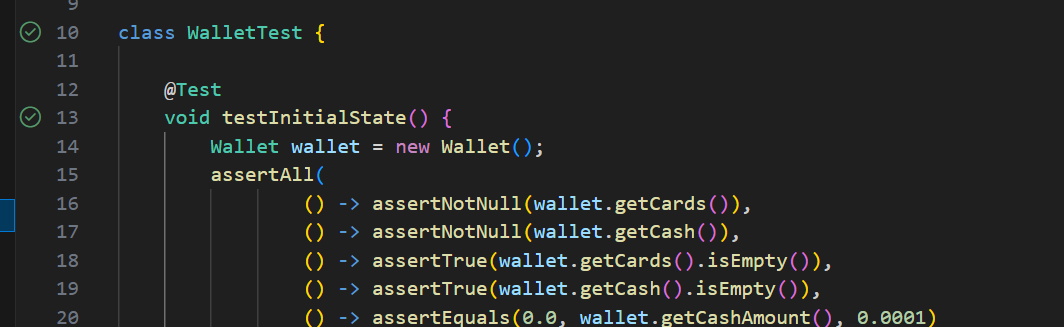
\includegraphics[width=0.9\textwidth]{resource/run-test-wallet.png}
    \caption{Menjalankan unit test WalletTest pada VS Code}
    \label{fig:run-test-wallet}
\end{figure}

\begin{figure}[H]
    \centering
    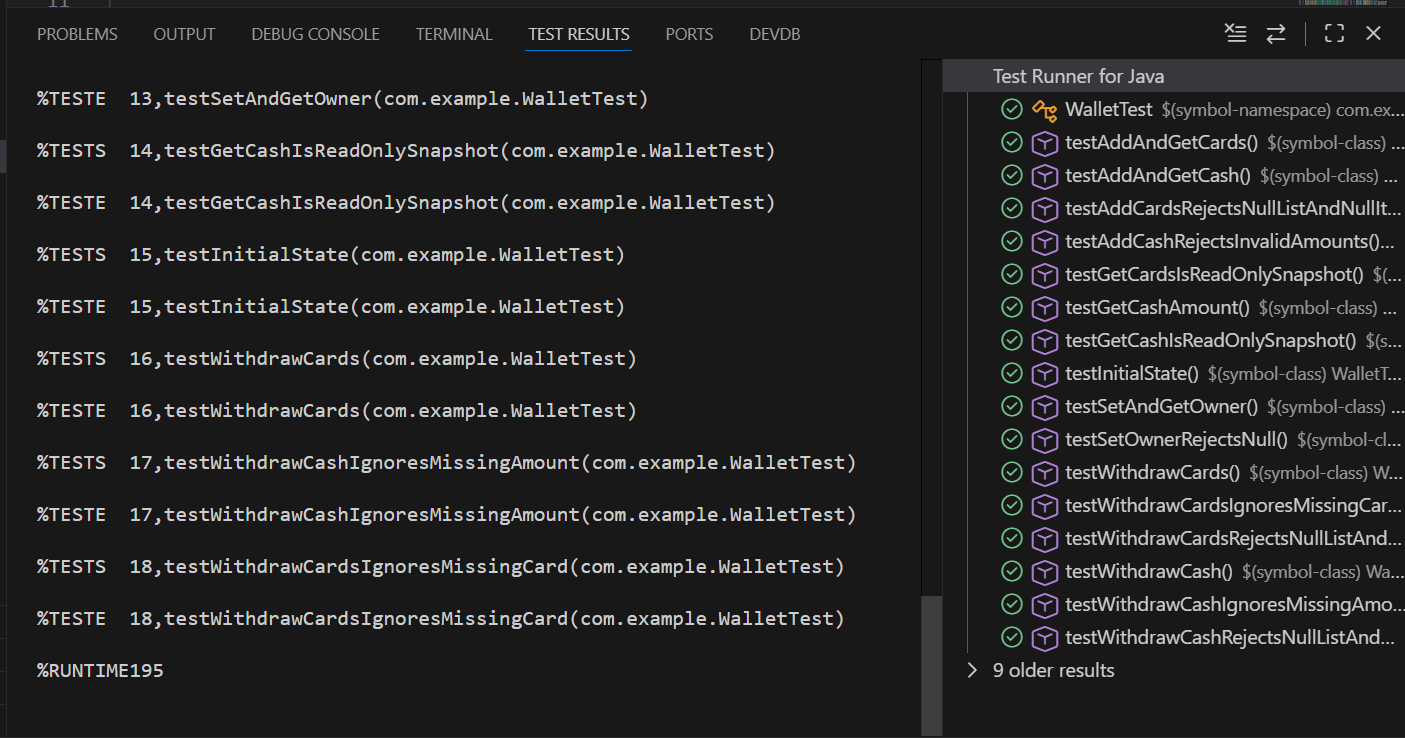
\includegraphics[width=0.9\textwidth]{resource/test-result-wallet.png}
    \caption{Hasil unit testing menunjukkan seluruh test case lulus (passed)}
    \label{fig:test-result-wallet}
\end{figure}

\section{Kesimpulan}
\par Berdasarkan hasil praktikum yang telah dilakukan, penerapan unit testing menggunakan JUnit 5 pada kelas \textit{Wallet} berhasil dilakukan sesuai dengan fungsionalitas yang saya implementasikan, yaitu pengelolaan data kartu (penambahan dan penghapusan), pengelolaan data uang tunai berbasis list nominal, serta perhitungan total saldo melalui method \textit{getCashAmount}. Pengujian dilakukan dengan mengidentifikasi skenario positif dan negatif, terutama untuk validasi input seperti parameter null, elemen list null, serta nominal uang yang tidak valid (nol dan negatif).

\par Selain itu, saya juga memastikan aspek \textit{immutability} pada data yang diekspos oleh objek dengan menguji bahwa \textit{getCards} dan \textit{getCash} mengembalikan snapshot yang bersifat read-only (tidak dapat dimodifikasi langsung). Penggunaan berbagai assert seperti \textit{assertAll}, \textit{assertIterableEquals}, \textit{assertThrows}, dan \textit{assertDoesNotThrow} membantu memastikan bahwa setiap method bekerja sesuai dengan perilaku yang diharapkan dan tahan terhadap input yang tidak sesuai. Dengan demikian, praktikum ini berhasil mencapai tujuan untuk memahami konsep unit testing dan menerapkannya menggunakan JUnit pada proyek Java berbasis Maven.

\end{document}